下表是某班一次数学测验的成绩统计表,请填上表中空缺部分,并根据上表中内容补全下面的条形统计图.
\[\begin{array}{|c|c|c|c|c|c|}
     \hline
    \text{分数} & 100 & 99\verb|-|90 & 89\verb|-|80 & 79\verb|-|70 & 69\verb|-|60 \\ \hline
    \text{人数} & 1   & 12    &       & 10    &       \\ \hline
    \text{占总人数的百分比} &  & 24\% & 38\% &  & 16\% \\ \hline

\end{array}\]

\begin{center}
    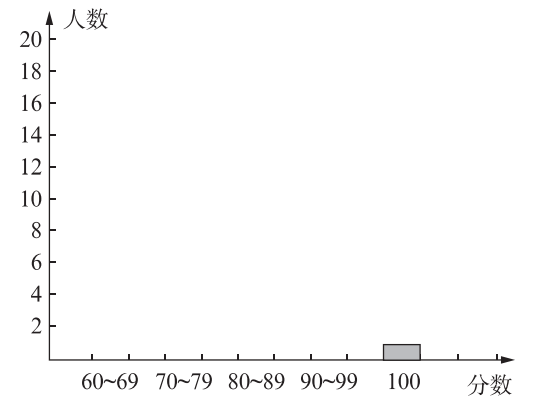
\includegraphics[height=6cm]{lib/image/MJA03050212.png}
\end{center}